\documentclass[14pt,a4paper,report]{report}
\usepackage[a4paper, mag=1000, left=2.5cm, right=1cm, top=2cm, bottom=2cm, headsep=0.7cm, footskip=1cm]{geometry}
\usepackage[utf8]{inputenc}
\usepackage[english,russian]{babel}
\usepackage{indentfirst}
\usepackage[dvipsnames]{xcolor}
\usepackage[colorlinks]{hyperref}
\usepackage{listings} 
\usepackage{fancyhdr}
\usepackage{caption}
\usepackage{graphicx}
\hypersetup{
	colorlinks = true,
	linkcolor  = black
}

\usepackage{titlesec}
\titleformat{\chapter}
{\Large\bfseries} % format
{}                % label
{0pt}             % sep
{\huge}           % before-code


\DeclareCaptionFont{white}{\color{white}} 

% Listing description
\usepackage{listings} 
\DeclareCaptionFormat{listing}{\colorbox{gray}{\parbox{\textwidth}{#1#2#3}}}
\captionsetup[lstlisting]{format=listing,labelfont=white,textfont=white}
\lstset{ 
	% Listing settings
	inputencoding = utf8,			
	extendedchars = \true, 
	keepspaces = true, 			  	 % Поддержка кириллицы и пробелов в комментариях
	language = bash,            	 	 % Язык программирования (для подсветки)
	basicstyle = \small\sffamily, 	 % Размер и начертание шрифта для подсветки кода
	numbers = left,               	 % Где поставить нумерацию строк (слева\справа)
	numberstyle = \tiny,          	 % Размер шрифта для номеров строк
	stepnumber = 1,               	 % Размер шага между двумя номерами строк
	numbersep = 5pt,              	 % Как далеко отстоят номера строк от подсвечиваемого кода
	backgroundcolor = \color{white}, % Цвет фона подсветки - используем \usepackage{color}
	showspaces = false,           	 % Показывать или нет пробелы специальными отступами
	showstringspaces = false,    	 % Показывать или нет пробелы в строках
	showtabs = false,           	 % Показывать или нет табуляцию в строках
	frame = single,              	 % Рисовать рамку вокруг кода
	tabsize = 2,                  	 % Размер табуляции по умолчанию равен 2 пробелам
	captionpos = t,             	 % Позиция заголовка вверху [t] или внизу [b] 
	breaklines = true,           	 % Автоматически переносить строки (да\нет)
	breakatwhitespace = false,   	 % Переносить строки только если есть пробел
	escapeinside = {\%*}{*)}      	 % Если нужно добавить комментарии в коде
}

\begin{document}

\def\contentsname{Contents}

% Titlepage
\begin{titlepage}
	\begin{center}
		\textsc{Peter the Great St.Petersburg Polytechnic University\\[5mm]
			Department of Computer Systems \& Software Engineering}
		
		\vfill
		
		\textbf{Laboratory report №1\\[3mm]
			Discipline: «Information Security»\\[3mm]
			Theme: «Encryption and Signing with GPG, Gpg4win»\\[41mm]
		}
	\end{center}
	
	\hfill
	\begin{minipage}{.4\textwidth}
		Made by student:\\[2mm] 
		Boyarkin N.S.\\
		Group: 13541/3\\[5mm]
		
		Lecturer:\\[2mm] 
		Bogach N.V.
	\end{minipage}
	\vfill
	\begin{center}
		Saint-Petersburg\\ \the\year\ y.
	\end{center}
\end{titlepage}

% Contents
\tableofcontents
\clearpage

\chapter{Laboratory work №1}

\section{Work purpose}

Learn utilities, based on PGP technology, for encrypting and decrypting data.

\section{Task}

\begin{enumerate}
	\item Study the description and launch graphic tool Kleopatra
	\item Create a key pair with OpenPGP (File -> New Certificate)
	\item Export Certificate (File -> Export Certificate)
	\item Sign/Encrypt Files (File -> Sign/Encrypt Files)
	\item Load other users certificates
	\item Import a certificate, sign it
	\item Verify the signature
	\item Using your partner certificate encrypt, sign and send her a file
	\item Accept, check and decrypt a file from your partner
	\item Following the instructions in GNU Privacy handbook play with gpg by CLI,i.e. without graphic tool.
\end{enumerate}

\clearpage

\section{Work Progress}

\subsection{Introduction}

Pretty Good Privacy (PGP) is an encryption program that provides cryptographic privacy and authentication for data communication. PGP is used for signing, encrypting, and decrypting texts, e-mails, files, directories, and whole disk partitions and to increase the security of e-mail communications.

GnuPG is a hybrid-encryption software program because it uses a combination of conventional symmetric-key cryptography for speed, and public-key cryptography for ease of secure key exchange, typically by using the recipient's public key to encrypt a session key which is only used once. This mode of operation is part of the OpenPGP standard and has been part of PGP from its first version.

\subsection{Kleopatra frontend}

\subsubsection{Creating a new certificate}

Let's illustrate the stage of creating a new certificate (File -> New Certificate ...). The first stage is the choice standard for a key pair. In addition to OpenPGP, Kleopatra also supports X.509:

\begin{figure}[h!]
	\centering
	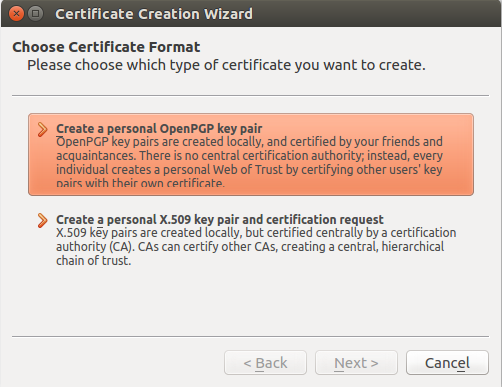
\includegraphics[scale = 0.65]{images/1_1.png}
	\caption{Select a standard for the key pair}
\end{figure}

After that, the process of configuring the certificate (selection of the encryption algorithm, length key, certificate name, etc.):

\begin{figure}[h!]
	\centering
	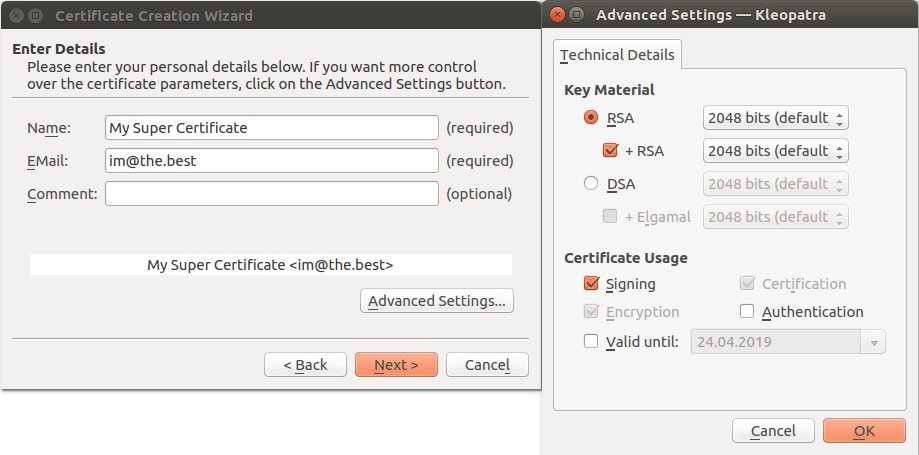
\includegraphics[scale = 0.65]{images/1_2.png}
	\caption{Configure the certificate and select the encryption algorithm}
\end{figure}

Then, the process of generating a pair of keys (based on random characters and the movement of the window) occurs, and the password for accessing the private key is set:

\begin{figure}[h!]
	\centering
	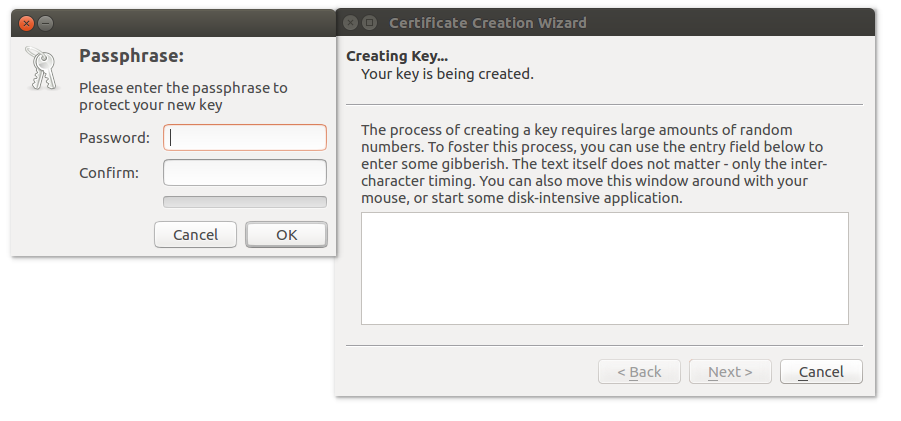
\includegraphics[scale = 0.65]{images/1_3.png}
	\caption{The process of generating a key pair and setting a password for accessing a private key}
\end{figure}

The generated certificate appears in the list of certificates:

\begin{figure}[h!]
	\centering
	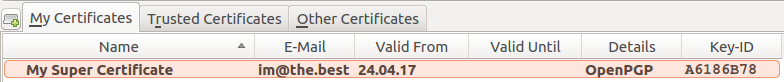
\includegraphics[scale = 0.7]{images/1_4.png}
	\caption{The result of creating a certificate}
\end{figure}

To obtain a public key, use the command MRC -> Export Certificate... Open key is stored in a file with it's own extension:

\begin{figure}[h!]
	\centering
	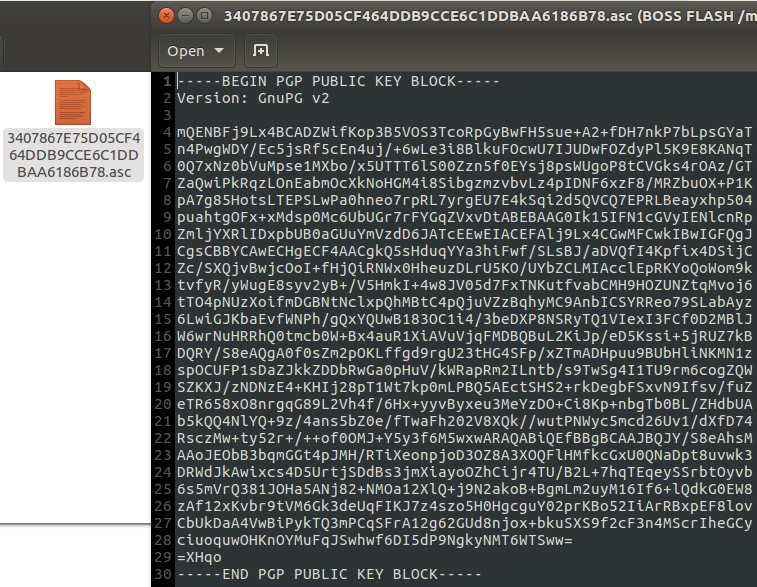
\includegraphics[scale = 0.65]{images/1_5.png}
	\caption{}
\end{figure}

\subsubsection{Encrypting}

On the \textbf{second} computer, we import a certificate (File -> Import Certificates ...), specifying as a parameter created public key:

\begin{figure}[h!]
	\centering
	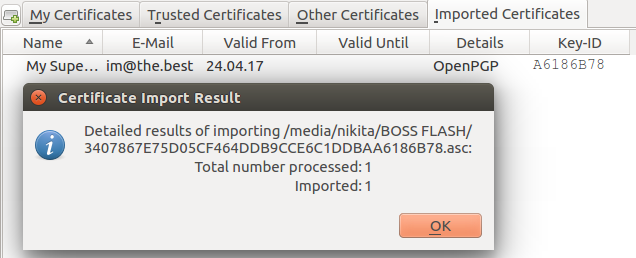
\includegraphics[scale = 0.55]{images/2_1.png}
	\caption{The result of importing the certificate on the second computer}
\end{figure}

To encrypt files, the command File -> Sign / Encrypt files was used ... A window appears with the choice of encryption parameters:

\begin{figure}[h!]
	\centering
	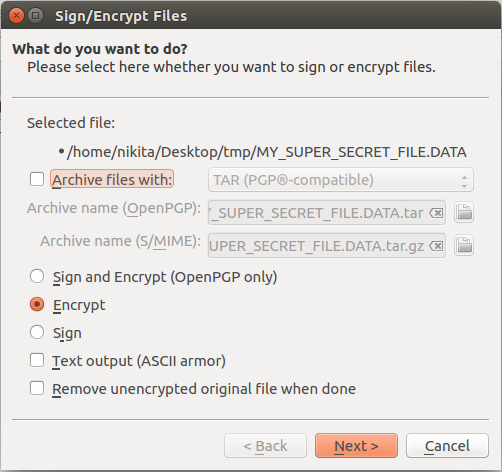
\includegraphics[scale = 0.53]{images/2_2.png}
	\caption{Choosing encryption options}
\end{figure}

The following is the certificate for encrypting the file:

\begin{figure}[h!]
	\centering
	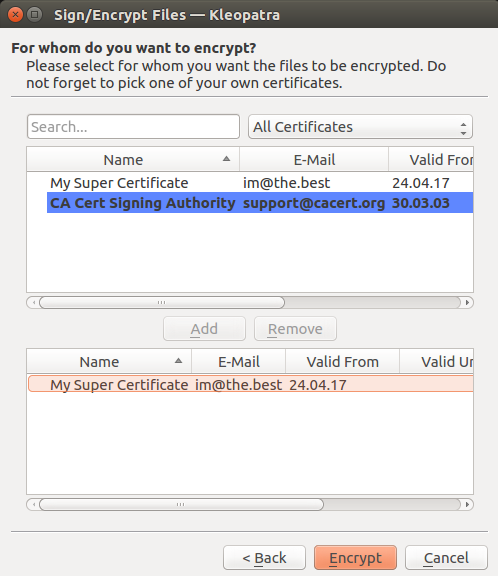
\includegraphics[scale = 0.53]{images/2_3.png}
	\caption{Choosing a certificate for encryption}
\end{figure}

The result of file encryption:

\begin{figure}[h!]
	\centering
	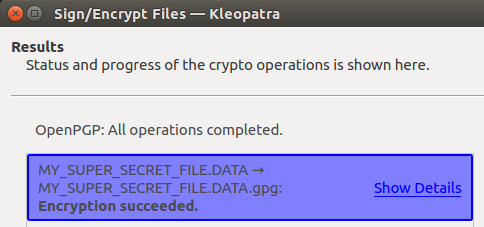
\includegraphics[scale = 0.6]{images/2_4.png}
	\caption{The result of file encryption}
\end{figure}

The file was encrypted in .gpg format, the decryption of this file is possible only with a private key, so you can not decrypt it on this computer, even considering that we encrypted it.

\subsubsection{Decrypting}

Transfer the .gpg file created on the second computer to the \textbf{first} (on which the certificate was created). To decrypt the files, we use the command File -> Decrypt / Verify files ... A window appears with the decoding parameters:

\begin{figure}[h!]
	\centering
	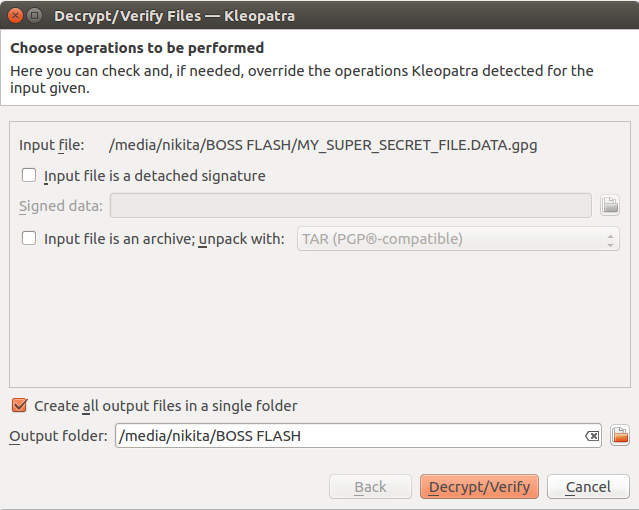
\includegraphics[scale = 0.48]{images/3_1.png}
	\caption{Selecting decryption options}
\end{figure}

To access the decryption with a private key, you must enter the password that was created with the certificate:

\begin{figure}[h!]
	\centering
	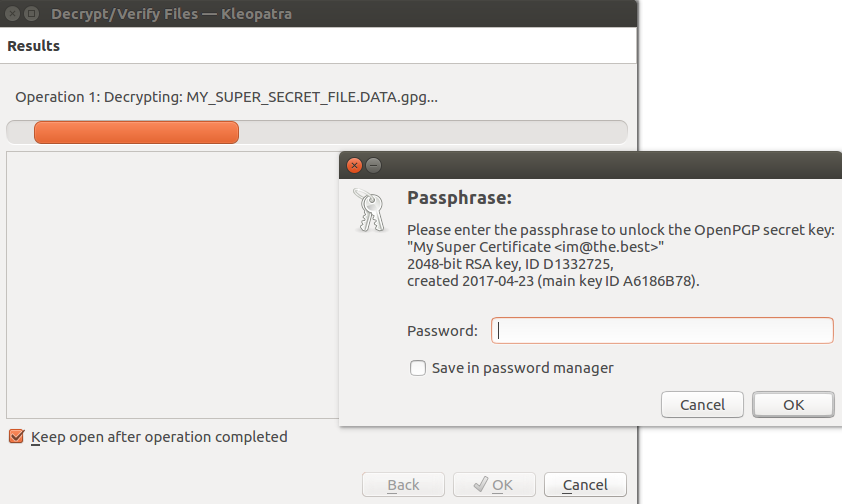
\includegraphics[scale = 0.48]{images/3_2.png}
	\caption{Explanation by the private key}
\end{figure}

The result of decrypting the file:

\begin{figure}[h!]
	\centering
	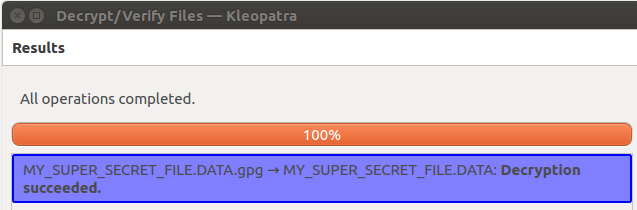
\includegraphics[scale = 0.6]{images/3_3.png}
	\caption{The result of decrypting the file}
\end{figure}

The file was successfully decrypted: the name and contents of the file are the same as the original.

\subsection{GPG command line}

\subsubsection{Symmetric-key encrypting}

For symmetric encryption, the -c flag is used:

\lstinputlisting{listings/sym.enc.log}

To decrypt a file, the combination of the -o and -d flags is used:

\lstinputlisting{listings/sym.dec.log}

\subsubsection{Public-key encrypting}

At the first step we creating and export the certificate by the following commands:

\lstinputlisting{listings/asym.cre.log}

Encrypting file on the second machine by the public key:

\lstinputlisting{listings/asym.enc.log}

The result of decrypting the file on the first machine:

\lstinputlisting{listings/asym.dec.log}

\section{Conclusion}

In this paper, we examined asymmetric encryption using the Kleopatra program of the OpenPGP family. Asymmetric encryption has the advantage over symmetric in the ease of exchange keys, but loses in encryption speed. The encryption considered in this work is one-way. In order to carry out two-way transmission, two channels are used. In modern cryptosystems, asymmetric encryption is used for key exchange, and at the same time symmetric encryption for data exchange.

\end{document}